%cc/cv de overleaf.com :s
\documentclass{beamer}
\usetheme{Frankfurt}
\usecolortheme{seahorse}
\title{Super titre de TIPE}
\subtitle{sous-titre}
\author{Alexandrine, Pedro\\\and De Carvalho, Enzo}
\date{2020-2021}

\usepackage{xurl}
\usepackage{graphicx}
\graphicspath{ {figures/} }

\begin{document}

\begin{frame}
	\maketitle
\end{frame}

\begin{frame}
	\frametitle{Sommaire}
	\tableofcontents
\end{frame}

\section{Première approche : simple regression}
\subsection{Principe}
\begin{frame}
	\frametitle{Principe de l'apprentissage supervisée}
	Donné une fonction $f : X \rightarrow y$ ($X$ et $y$ des données corrélées), un algoritmhe d'apprentissage supervisé cherche alors à obtenir un modèle $g : X \rightarrow y$ qui estime $f$ à partir d'une d'une partie $Y \subset f(X)$ déjà connue de l'algoritme.
	\begin{figure}[b]
		\centering
		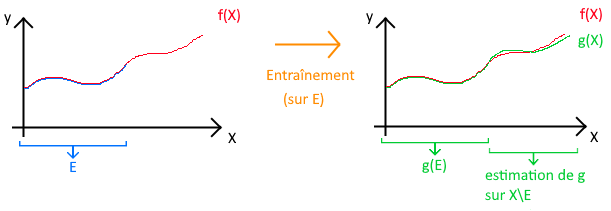
\includegraphics[scale=0.65]{super_schema}
	\end{figure}
\end{frame}

\begin{frame}
	\frametitle{Principe de l'apprentissage supervisée}
	La création du modèle passe par l'optimisation d'une fonction d'objectif, où les paramètres à optimiser sont ceux du modèle.
	Exemple avec une regression linéaire dont le modèle est de la forme :
	\begin{figure}[h]
		\centering
		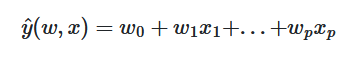
\includegraphics[scale=0.7]{f_lineair}
		\caption{$x$ les données, $w$ les paramètres}
	\end{figure}
	\alert{N.B : refaire la figure (celle-ci est volée du manuel scikit)}
\end{frame}

\begin{frame}
	\frametitle{ElasticNet}
	La fonction d'objectif d'ElasticNet minimise : (à l'aide d'un algorithme itératif "Coordinate Descent" (trad?))
	\begin{figure}[h]
		\centering
		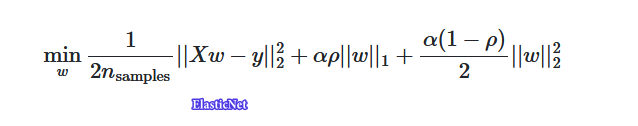
\includegraphics[scale=0.4]{fonction_dobj}
		\caption{$\alpha$ et $\rho$ sont des hyperparamètres définissant le modèle}
	\end{figure}
	\begin{figure}[b]
		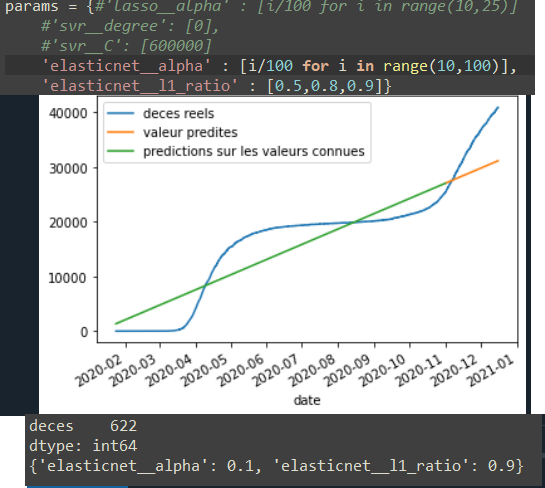
\includegraphics[scale=0.2]{EN}
		\centering
		\caption{résultats peu intéressant dans notre cas..}
	\end{figure}
\end{frame}

\subsection{Optimisation d'hyperparamètres et stratégies}
\subsubsection{Cross-validation}
\begin{frame}
	\frametitle{Recherche du meilleur paramètre}
	On recherche la meilleur combinaison des paramètres donnés en évaluant successivement chaque modèle pour chacune des combinaisons possibles selon une stratégie de "cross-validation" :
	\begin{figure}[b]
		\centering
		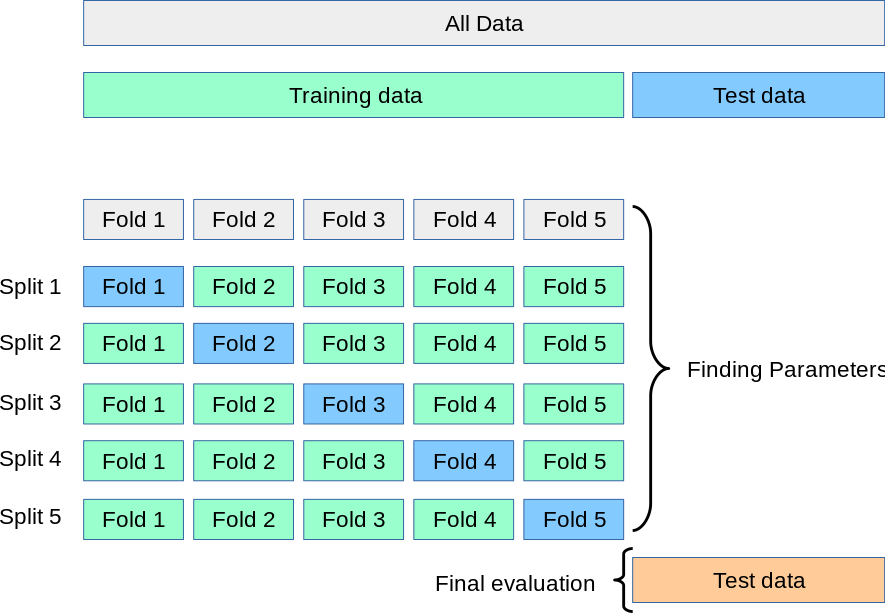
\includegraphics[scale=0.2]{gscv}
	\end{figure}
\end{frame}

\subsection{Résultats avec SVR}
\begin{frame}
	\frametitle{SVR ; premier résultat}
	Approche à l'aide du modèle SVR (avec le noyau 'rbf') (Support Vector Regressor)
	\begin{figure}[tc]
		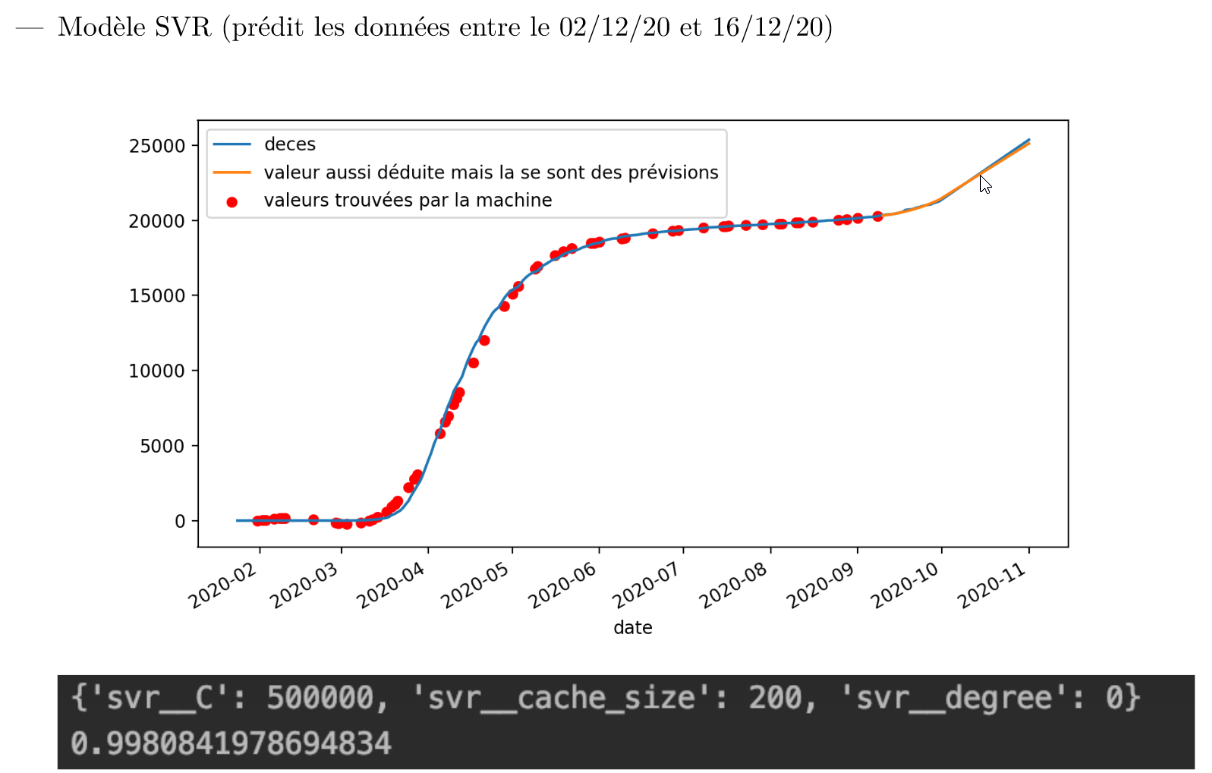
\includegraphics[scale=0.2]{SVR_premierdecoup}
		\centering
		\caption{Premier résultat avec SVR avec une "mauvaise stratégie" de découpage pour former un modèle prédisant une série temporelle}
	\end{figure}
\end{frame}

\subsubsection{Découpages adaptés}
\begin{frame}
	\frametitle{Découpage adapté pour la CV}
		Une note moyenne est donnée à un set de paramètres selon un score moyen donné sur chacun des découpages.
		Pour une évaluation cohérente, il faut un découpage cohérent :
		\begin{figure}[h]
			\centering
			\begin{minipage}{0.4\textwidth}
				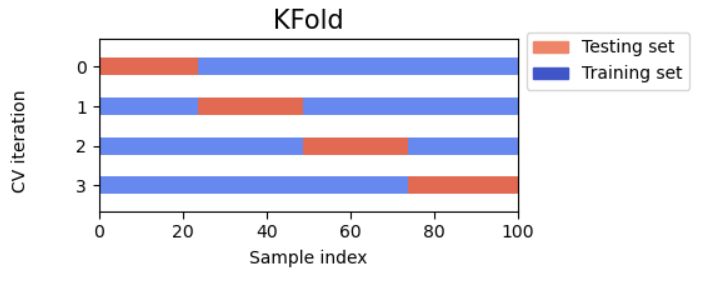
\includegraphics[scale=0.25]{kfold}
			\end{minipage}
			\begin{minipage}{0.4\textwidth}
				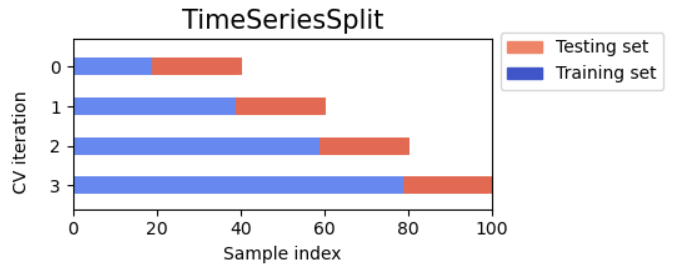
\includegraphics[scale=0.25]{tscv}
			\end{minipage}
		\caption{Comparaison des différents découpages des données employés pour la CV}
		\end{figure}
\end{frame}

\begin{frame}
	\frametitle{SVR}
	\begin{figure}[t]
		\centering
		\begin{minipage}{0.5\textwidth}
			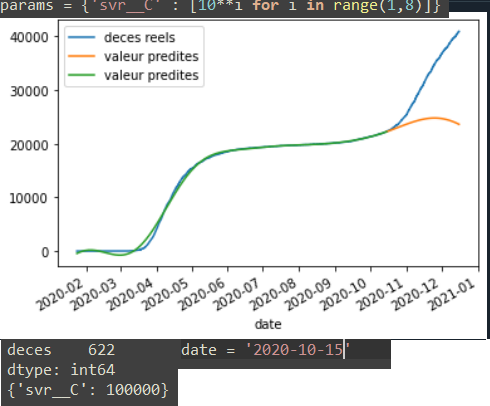
\includegraphics[scale=0.25]{SVR_avant_pt_dinflexion}
		\end{minipage}%
		\begin{minipage}{0.5\textwidth}
			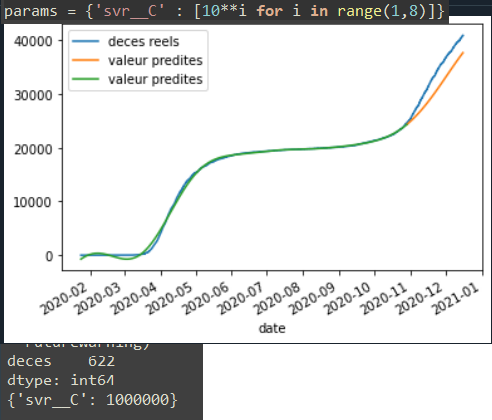
\includegraphics[scale=0.25]{SVR_apres_pt_dinflexion}
		\end{minipage}
	\caption{à gauche la prediction avant le pt d'inflexion, à droite, après.}
	\end{figure}
	$\Rightarrow$ Le modèle n'arrive pas à "suivre" sans le point d'inflexion.
\end{frame}
\begin{frame}
	\frametitle{fbprophet}
	Approche avec le module fbprophet (designé pour prédire des séries temporelles)
	\begin{figure}[t]
		\begin{minipage}{0.3\textwidth}
			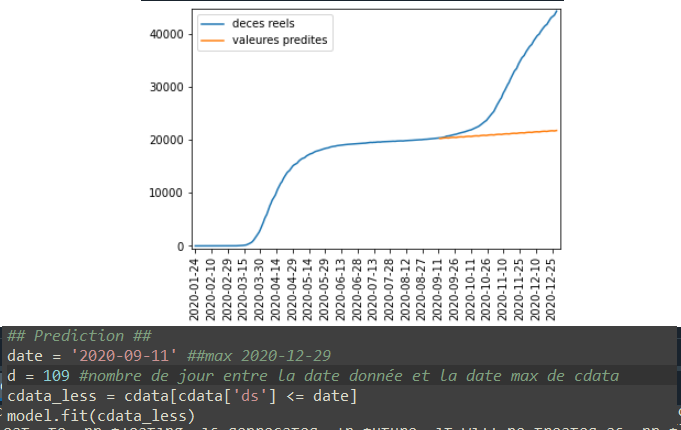
\includegraphics[scale=0.13]{fbprophet_avant_pt_dinflexion}
		\end{minipage}
		\begin{minipage}{0.3\textwidth}
			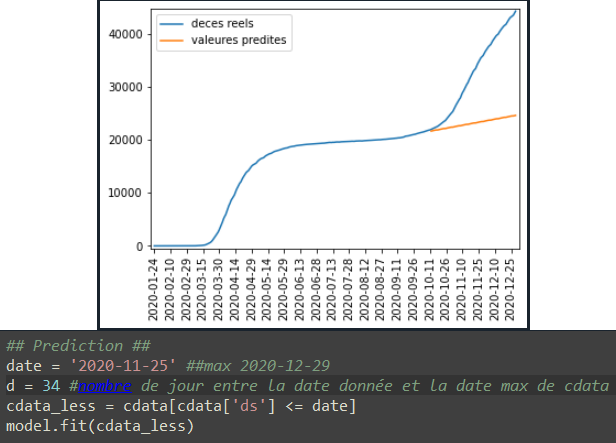
\includegraphics[scale=0.13]{fbprophet_mid_pt_dinflexion}
		\end{minipage}
		\begin{minipage}{0.3\textwidth}
			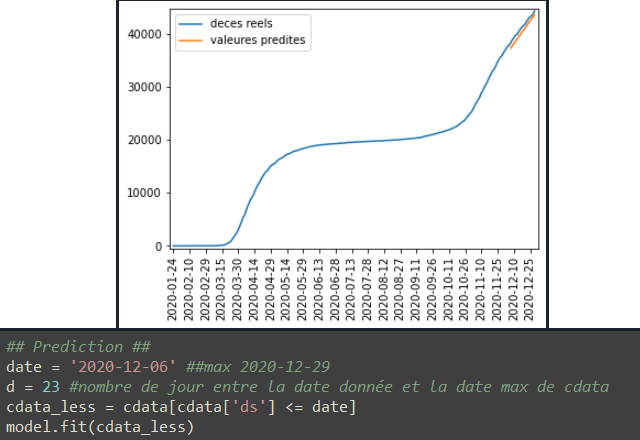
\includegraphics[scale=0.13]{fbprophet_apres_pt_dinflexion}
		\end{minipage}
	\caption{résultats avec fbprophet (insatisfaisant)}
	\end{figure}
\end{frame}

\section{Approche multivariées}
\subsection{Multiregresseur : 'RegressorChain'}
\begin{frame}
	\frametitle{RegressorChain SVR}
	Approche avec le multiregresseur\\
	\tiny{(description de scikit : \url{https://scikit-learn.org/stable/modules/generated/sklearn.multioutput.RegressorChain.html########sklearn.multioutput.RegressorChain})}\\
	\normalsize{\textit{"Each model makes a prediction in the order specified by the chain using all of the available features provided to the model plus the predictions of models that are earlier in the chain."}}
	\begin{figure}[h]
		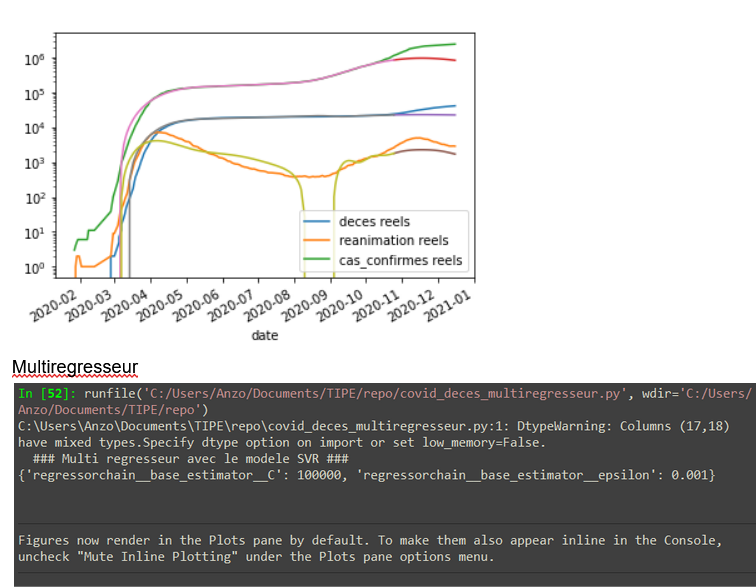
\includegraphics[scale=0.3]{mulitregr_epic_fail}
		\caption{résultat avec SVR (insatisfaisant)}
	\end{figure}
\end{frame}

\subsection{Réseau neuronal}
\begin{frame}
	\frametitle{Explications}
	\begin{figure}[t]
		\centering
		\begin{minipage}{0.5\textwidth}
			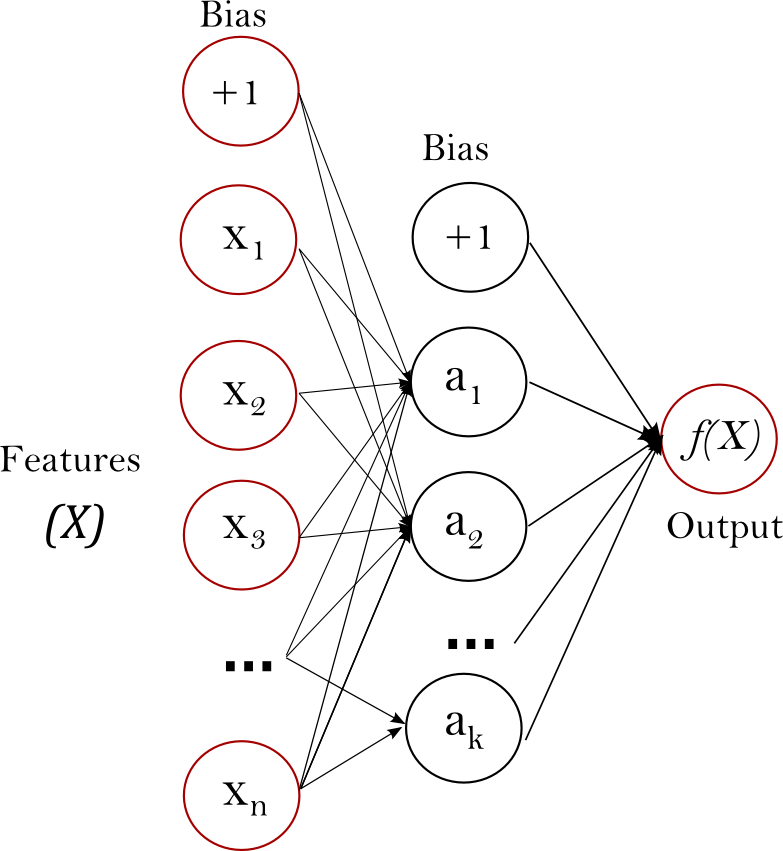
\includegraphics[scale=0.15]{nn_sk}
		\end{minipage}
		\begin{minipage}{0.3\textwidth}
			\tiny{Basé sur le fonctionnement du cerveau. Donne un jeu de donné successivement interprétées par un jeu de hidden layers. Un hidden layer est un jeu de neurones chacun interprétant et transformant les objets donnés pour décrypter le jeu de donnés précédents. À la fin on aboutit au résultat trouvé par la machine. Le but de l'entrainement ici est l'ajustement de chaque hidden layer et de ces neurones pour tomber sur des prédictions les plus proches possible de la réalité. $Maxiter$ est alors le nombre de fois que le modèle va s'entrainer au maximum si il n’a pas réussi à aboutir à un résultat satisfaisant la tolérance tol donnée.}
		\end{minipage}
	\\
	\alert{N.B trop verbeux !}
	\end{figure}
\end{frame}

\begin{frame}
	\frametitle{Résultats}
	\begin{figure}[h]
		\centering
		\begin{minipage}{0.5\textwidth}
			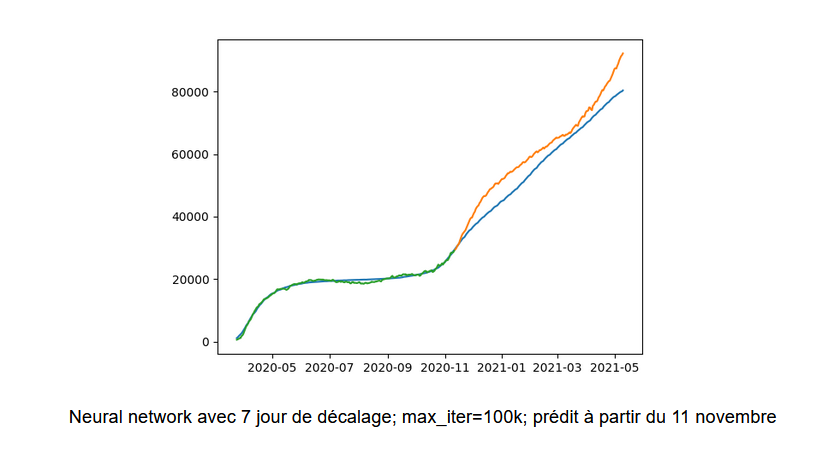
\includegraphics[width=\textwidth]{NN_1}
			\centering
		\end{minipage}
		\begin{minipage}{0.5\textwidth}
			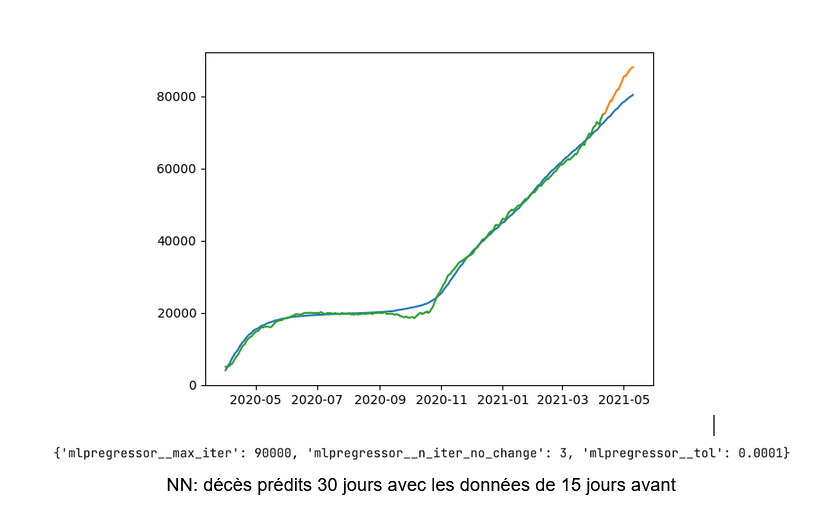
\includegraphics[width=\textwidth]{NN_2}
			\centering
		\end{minipage}
	\end{figure}
\end{frame}

\begin{frame}
	\frametitle{Résultats}
	\begin{figure}
		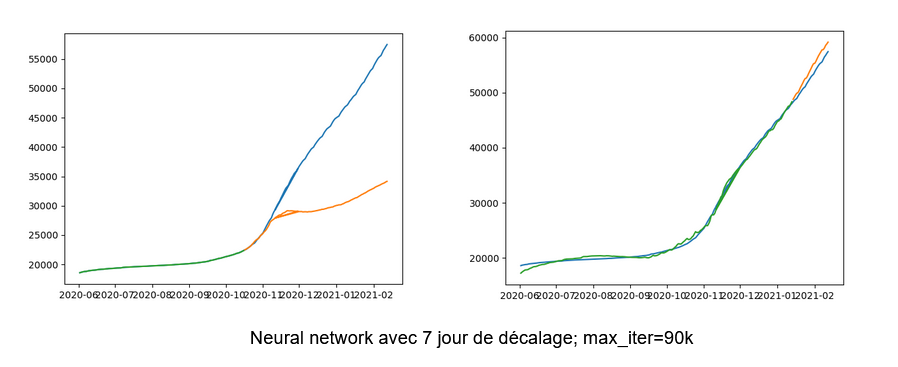
\includegraphics[scale=0.6]{NN_3}
		\caption{échec du modèle sans la courbe des cas confirmés}
	\end{figure}
\end{frame}

\begin{frame}
	\frametitle{Notes}
	\alert{N.B les diapos sont trop verbeux; il faut encore un effort de concision, ou alors elles doivent être expliquées à l'oral}\\
	\alert{N.B sourcer les images}
\end{frame}

\end{document}
